% =====================================================================
%  第 6 章 §6.5 后半（原书 p.320–332 / PDF 330–342）—— ch06c2
%  续写；不写章标题、不写节标题（已在 ch06c.tex 中）
% =====================================================================

% [原文 p.320]
（不过要注意，$\circ$ 并不结合。）
% [Tutor Note: 本行是原书 p.319 末开始、p.320 页首结束的括号说明的结尾（ch06c 已先行闭合 proof 环境）；合稿时可视需要并入 ch06c 末句。]

下面证明 $\rd[f,g]=[\rd f,g]+(-1)^f[f,\rd g]$。令 $h(a_1,a_2)=a_1\cdot a_2$（$\cdot$ 为 $A$ 的积），则 $\rd f=[h,f]$。因此 $\rd[f,g]=[\rd f,g]+(-1)^f[f,\rd g]$ 也是（Gerstenhaber 括号的）Jacobi 律。

\begin{lemma*}{6.161}
  设 $\Psi\in\Pi^2C^0(A,A)=\mathrm{Hom}(A^{\otimes2},A)$。$f*g=fg+\Psi(f,g)$ 结合的必要充分条件由下式表出：
  \begin{equation}
    \rd\Psi+\frac12[\Psi,\Psi]=0. \tag{6.61}
  \end{equation}
\end{lemma*}
\begin{proof}
  \begin{align*}
    &f*(g*h)-(f*g)*h\\
    &\quad=fgh+\Psi(f,g)h+\Psi(fg,h)+\Psi(\Psi(f,g),h)\\
    &\qquad-fgh-f\Psi(g,h)-f\Psi(g,h)-\Psi(f,gh)-\Psi(f,\Psi(g,h))\\
    &\quad=(\rd\Psi)(f,g,h)+\frac12[\Psi,\Psi](f,g,h).
  \end{align*}
\end{proof}

(6.61) 是 §6.4 所论 Maurer–Cartan 方程的一种。设 $A=C^\infty(M)\otimes\R[[T]]$。

\begin{definition}{6.162}
  把多重线性微分作用素的、关于 $T$ 的形式幂级数即 $C^k(A,A)$ 的元全体记作 $CD^k(A,A)$。即 $\Psi\in CD^k(A,A)$ 可表为
  \[
    \Psi(f_0,\dots,f_k)=\sum_{I_0,\dots,I_k}\alpha^{I_1,\dots,I_k}_m\partial_{I_0}f_1\cdots\partial_{I_k}f_kT^m.
  \]
  这里 $I_j=(i^j_1,\dots,i^j_{|I_j|})$ 是多重指标，$\partial_{I_j}f$ 由下式定义：
  \[
    \partial_{I_j}f=\frac{\partial^{|I_j|}f}{\partial x^{i^j_1}_j\cdots\partial x^{i^j_{|I_j|}}_j}.
  \]
\end{definition}

下面的引理证明容易。

\begin{lemma}{6.163}
  $CD^*(A,A)$ 关于 $\rd$ 与 Gerstenhaber 括号是封闭的。
\end{lemma}
% [Tutor Note: $CD^k(A,A)$ 是 Hochschild 上链的“微分作用素版本”：普通的 Hochschild 上链只允许 $\Psi(f_1,\dots,f_k)$ 是函数的乘法组合，这里允许对 $f_i$ 求任意阶偏导，并带 $T$ 的幂级数。Kontsevich 的形变量子化正是在这个更大的代数里解 Maurer–Cartan 方程。]

以后考察 $\Pi^2CD(A,A)$。应当证明的是：方程 (6.61) 有足够多

% [原文 p.321]
的解。(6.61) 是关于 Gerstenhaber 括号的。另一方面，Poisson 结构由引理 6.158 与 Schouten 括号相联系。考察 Gerstenhaber 括号所定微分李代数与 Schouten 括号所定微分李代数的关系，正是 Kontsevich 问题 1.10 的肯定解决的方法。首先，在这两者之间作映射。不过这个映射不是微分李代数的同态。

\begin{definition}{6.164}
  对 $\alpha=\sum\alpha^I\partial_{i_1}\wedge\dots\wedge\partial_{i_{|I|}}\in\Gamma(M;\Omega^k(M))$，由下式定义 $\varphi_1(\alpha)\in CD^k(A,A)$：
  \[
    \varphi_1(\alpha)(f_1\cdots f_k)=\frac1{k!}\sum_{\sigma\in\mathfrak{S}_k}\sum_I\mathrm{sign}(\sigma)\alpha^I\partial_{i_1}f_{\sigma1}\wedge\dots\wedge\partial_{i_k}f_{\sigma k}.
  \]
\end{definition}

\begin{lemma}{6.165}
  $\iota_1\varphi_1=0$。
\end{lemma}

由于 $\Gamma(M;\Omega M)$ 上没有微分，引理 6.165 意味着 $\varphi_1$ 是链映射。引理 6.165 的证明代入定义即得，故省略。

下一定理是 [221] 的主定理，在 [220] 中被称为形式性猜想（formality conjecture）。

\begin{theorem}{6.166}
  （Kontsevich）存在 $\varphi_k:E_k\Pi^2(\Gamma(M;\Omega(M)))\to\Pi^2CD(A,A)$，$k=2,\dots$，且 $\varphi$ 是 $L_{\infty}$ 写像。
\end{theorem}
% [Tutor Note: 形式性定理的要点是：$\Gamma(M;\Omega(M))$ 上由 Schouten 括号给出的微分分次李代数，与 $CD(A,A)$ 上由 Gerstenhaber 括号给出的微分分次李代数，二者的同调相同（$\varphi_1$ 诱导同型），且可提升为 $L_{\infty}$ 拟同构 $\varphi$。正因如此，Schouten 括号意义下的 Poisson 结构可以直接“搬运”为结合积。]

\begin{remark}{6.167}
  比较容易证明 $\varphi_1$ 在同调上诱导同型（[221]）。因此定理 6.166 的 $L_{\infty}$ 写像是同伦等价。
\end{remark}

由定理 6.166，可导出对任意 Poisson 结构的形变量子化的存在。

\begin{theorem}{6.168}
  设 $\{\cdot,\cdot\}$ 为 $M$ 上的 Poisson 结构。则存在结合积 $*:C^\infty(M)[[T]]^2\to C^\infty(M)[[T]]$，使 $f*g=fg+\{f,g\}T\ \mathrm{mod}\ T^2$ 成立。
\end{theorem}

\begin{proof}[定理 6.166 $\Rightarrow$ 定理 6.168 的证明]
  设 $\{f,g\}=\sum\omega^{ij}\partial_if\partial_jg$。则 $\alpha=\sum\omega^{ij}\partial_i\wedge\partial_j\in\Gamma(M;\Omega^k(M))$，而由引理 6.158，$\iota_2(\alpha,\alpha)=0$。换言之，$\hat\rd e^\alpha=0$。
% [原文 p.322]
  令
  \[
    \Psi=\sum_{k=1}^\infty\frac1{k!}\varphi_k(\alpha,\dots,\alpha)T^k\in CD^2(A,A)[[T]].
  \]
  换言之，$\hat\varphi(e^\alpha)=e^\Psi$。因此 $\hat\rd(e^\Psi)=\hat\varphi(\hat\rd e^\alpha)=0$。即 (6.61) 成立。于是由引理 6.161，$f*g=fg+\Psi(f,g)$ 是结合积。$\Psi$ 关于 $T$ 的 1 次部分是 $\varphi_1(\alpha)$，按定义它就是 Poisson 括号。
\end{proof}

本节余下的部分叙述定理 6.166 证明的概要。只说明 $M$ 为 $\R^n$ 的情形。一般情形请看原论文 [221]。

设 $\alpha_i\in\Gamma(M;\Omega^{m_i}(M))$。$\alpha_i$ 的次数移动后为 $m_i-2$，而 $\varphi_k$ 的次数为 $0$。因此 $\varphi_k(\alpha_1,\dots,\alpha_k)\in\Pi^2CD(A,A)$ 的（移动前的）次数是 $m=\sum m_i-2k+2$。于是取 $m$ 个函数 $f_1,\dots,f_m$，想定义
\begin{equation}
  \varphi_k(\alpha_1,\dots,\alpha_k)(f_1,\dots,f_m). \tag{6.62}
\end{equation}
(6.62) 由关于满足以下条件的图 $\Gamma$ 之和来定义。$\Gamma$ 是边与顶点带编号、边带方向的图。
\begin{enumerate}[label=（\arabic*）]
  \item $\Gamma$ 有 $k+m$ 个顶点 $p_1,\dots,p_k$ 与 $q_1,\dots,q_m$。
  \item 以 $p_i$ 为起点的边恰好有 $m_i$ 条。给它们命名为 $e^i_1,\dots,e^i_{m_i}$。没有以 $q_i$ 为起点的边。
  \item $e^i_1,\dots,e^i_{m_i}$ 的终点互不相同。又 $p_i$ 也不是任何 $e^i_1,\dots,e^i_{m_i}$ 的终点。
\end{enumerate}
把满足 (1)、(2)、(3) 的图全体记作 $\mathfrak{T}(k;m_1,\dots,m_k;m)$。（这里说“图”时，已把边的定向、边与顶点的编号都包含在内。）

设给定 $\mathfrak{T}(k;m_1,\dots,m_k;m)$ 的元 $\Gamma$。对每个 $e^i_j$ 分配 $1$ 到 $n$ 中的某个指标 $\ell^i_j$。把它们合起来记作 $\vec\ell$。

对 $\Gamma\in\mathfrak{T}(k;m_1,\dots,m_k;m)$，按下述规则定义函数 $U_\Gamma(\vec\ell)(\alpha_1,\dots,\alpha_k)(f_1,\dots,f_m)$。令 $\alpha_i=\sum\alpha^{a(1),\dots,a(m_i)}_i\partial_{a(1)}\wedge\dots\wedge\partial_{a(m_i)}$，并令 $\alpha_i(\vec\ell)=\alpha^{\ell^i_1,\dots,\ell^i_{m_i}}_i$。取 $\alpha_i(\vec\ell)$（$i=1,\dots,k$）与 $f_1,\dots,f_m$，施行下列操作。
\begin{enumerate}[label=（\arabic*）]
  \item 若 $e^i_j$ 的终点为 $p_{i'}$，则让 $\partial_{\ell^i_j}$ 作用于 $\alpha_{i'}(\vec\ell)$。
  \item 若 $e^i_j$ 的终点为 $q_{i'}$，则让 $\partial_{\ell^i_j}$ 作用于 $f_{i'}$。
\end{enumerate}
这样得到的 $\alpha_i(\vec\ell)$ 的微分与 $f_i$ 的微分全部相乘所得者，

% [原文 p.323]
就是 $U_\Gamma(\vec\ell)(\alpha_1,\dots,\alpha_k)(f_1,\dots,f_m)$。然后定义
\[
  U_\Gamma(\alpha_1,\dots,\alpha_k)(f_1,\dots,f_m)=\frac1{m!}\sum_{\vec\ell}U_\Gamma(\vec\ell)(\alpha_1,\dots,\alpha_k)(f_1,\dots,f_m).
\]
例如，图 6.11(a) 的情形是
\[
  \resizebox{0.97\linewidth}{!}{$\displaystyle U_\Gamma(\alpha_1,\alpha_2,\alpha_3,\alpha_4)(f_1,f_2,f_3)=\frac16\sum\frac{\partial\alpha^{\ell^1_1\ell^1_2}_1}{\partial x_{\ell^2_2}}\frac{\partial\alpha^{\ell^2_1\ell^2_2}_2}{\partial x_{\ell^2_1}}\frac{\partial\alpha^{\ell^3_1\ell^3_2}_3}{\partial x_{\ell^3_2}}\frac{\partial\alpha^{\ell^4_1\ell^4_2}_4}{\partial x_{\ell^3_1}}\frac{\partial f_1}{\partial x_{\ell^1_1}}\frac{\partial^2f}{\partial x_{\ell^4_1}\partial x_{\ell^2_2}}\frac{\partial f_3}{\partial x_{\ell^3_1}}. $}
\]
而图 6.11(b) 的情形是 $\varphi_1(\alpha)(f_1,\dots,f_m)$。

\begin{figure}[htbp]
  \centering
  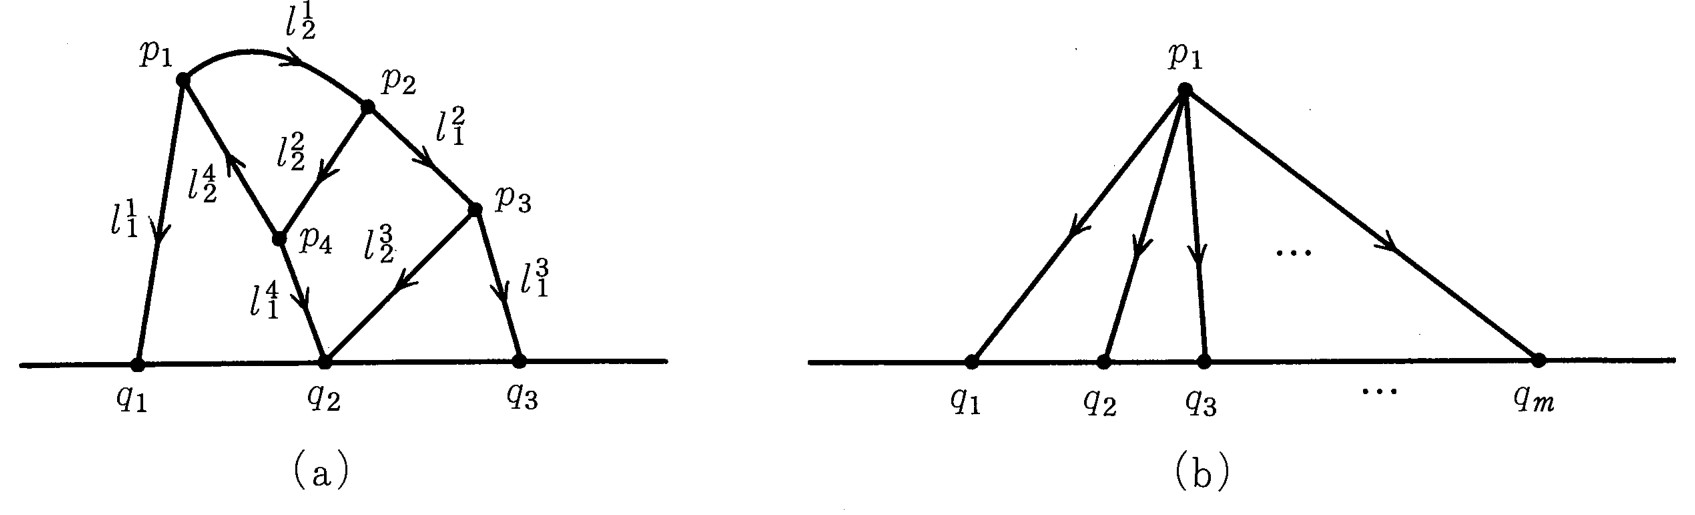
\includegraphics[width=0.80\textwidth]{figures/fig6.11.png}
  \figtitle{6.11}{$U_\Gamma$ 的例子（原书 p.323）}
\end{figure}

其次定义权 $W(\Gamma)\in\R$。令 $m=\sum m_i-2k+2$。首先如下定义 $\hat C(k,m)$。考虑上半平面 $\HH=\{z\in\C\mid \mathrm{Im}\,z\ge0\}$ 与其边界 $\R$。对顶点 $p_i$ 取 $\HH$ 的元 $z_i$，对 $q_i$ 考虑 $\R$ 的点 $w_i$。不过 $z_i$ 们与 $w_i$ 们全都互不相同。$\hat C(k,m)$ 为这样的点组 $(z_1,\dots,z_k,w_1,\dots,w_m)$ 全体。$\dim\hat C(k,m)=2k+m$。由假定 $2k+m=\sum m_i+2$。即 $\dim\hat C(k,m)$ 是边数 $+2$。考虑变换 $z\mapsto cz+d$（$c\in\R_+$，$d\in\R$）全体 $G$。$G$ 的元把 $\HH$ 的元移到 $\HH$。因此 $G$ 作用在 $\hat C(k,m)$ 上。把其商空间记作 $C(k,m)$。$\dim C(k,m)=\sum m_i$。

设 $[z,\vec w]$ 为 $C(k,m)$ 的点，$e^i_j$ 为 $\Gamma$ 的边。$p_i$ 是 $e^i_j$ 的起点。设 $e^i_j$ 的终点为 $p_{i'}$。此时考虑连接 $z_i$ 与 $z_{i'}$ 的 $\HH$ 的测地线（关于双曲度量），它与连接 $z_i$ 与 $\infty$ 的 $\HH$ 的测地线之间的（带符号的）角

% [原文 p.324]
\begin{figure}[htbp]
  \centering
  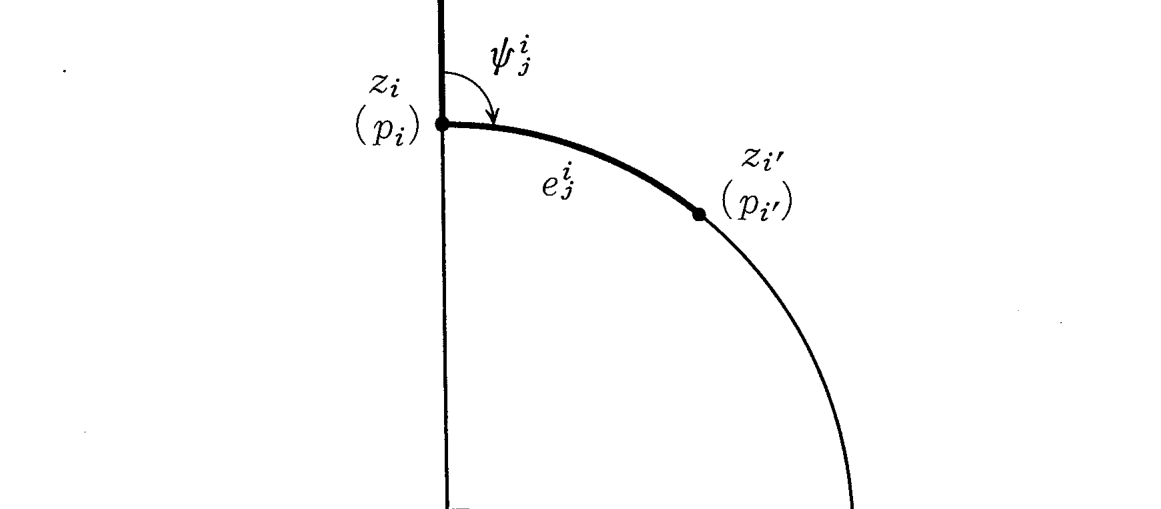
\includegraphics[width=0.42\textwidth]{figures/fig6.12.png}
  \figtitle{6.12}{$\psi^i_j$ 的定义（原书 p.324）}
\end{figure}

记作 $\psi^i_j([z,\vec w])\in\R/2\pi\Z$（图 6.12）。当 $e^i_j$ 的终点为 $q_{i'}$ 时，考虑连接 $z_i$ 与 $w_{i'}$ 的 $\HH$ 的测地线，同样定义 $\psi^i_j([z,\vec w])$。

$\rd\psi^i_j$ 是 $C(k,m)$ 上的微分 1-形式。
\begin{equation}
  W(\Gamma)=\frac{(2\pi)^{-(2k+m-2)}}{m_1!\cdots m_k!}\int_{C(k,m)}\prod_{i,j}\rd\psi^i_j \tag{6.63}
\end{equation}
（积分号内是微分 $\sum m_i$ 形式，而 $\dim C(k,m)=\sum m_i$，故积分的次数是相符的。$C(k,m)$ 不紧，但下一条引理成立。）

\begin{lemma}{6.169}
  (6.63) 的积分收敛。
\end{lemma}

证明随后立即给出。
% [Tutor Note: $W(\Gamma)$ 是 Kontsevich 型构型空间积分：$\bar C(k,m)$ 是上半平面上带“角参数”的紧化，$\rd\psi^i_j$ 是双曲测地线之间的角。积分收敛靠的是紧化后 $\rd\psi^i_j$ 的光滑延拓（引理 6.172）。]

\begin{remark}{6.170}
  (6.63) 中取的是微分 1-形式的积，故须慎重考虑符号；关于符号的讨论这里省略。
\end{remark}

\begin{definition}{6.171}
  如下定义 $\R^n$ 上的函数 $\varphi_k(\alpha_1,\dots,\alpha_k)(f_1,\dots,f_m)$：
  \[
    \varphi_k(\alpha_1,\dots,\alpha_k)(f_1,\dots,f_m)=\sum_{\Gamma\in\mathfrak{T}(k;m_1,\dots,m_k;m)}W(\Gamma)U_\Gamma(\alpha_1,\dots,\alpha_k)(f_1,\dots,f_m).
  \]
\end{definition}

$\varphi_k$ 确定映射 $E\Pi^2(\Gamma(M;\Omega^k(M)))\to\Pi^2CD(A,A)$。由于图 6.11(b) 表示 $\varphi_1$，$k=1$ 时定义 6.171 就是 $\varphi_1$。（对图 6.11(b) 的图 $\Gamma_m$，$W(\Gamma_m)=1$。）

% [原文 p.325]
定义 6.171 给出 $L_{\infty}$ 写像，这是定理 6.166 的主张。证明用 Stokes 定理进行。为了证明，构成 $C(k,m)$ 的紧化。

\begin{lemma}{6.172}
  存在 $C(k,m)$ 的紧化，即带角流形 $\bar C(k,m)$，且 $\rd\psi^i_j$ 是 $\bar C(k,m)$ 上光滑微分 1-形式的限制。
\end{lemma}

引理 6.169 由引理 6.172 立即得出。
\begin{proof}
  首先，把 $(z_1,\dots,z_k,w_1,\dots,w_m)\in C(k,m)$ 对应于 $M_{0,k+m+1}$ 的点 $(z_1,\dots,z_k,w_1,\dots,w_m,\infty)$。注意这个映射确定从 $C(k,m)$ 出发的单射。（把 $\HH$ 的自同构中固定无穷远点的，只有 $z\mapsto az+b$ 形的。）于是考虑 $C(k,m)$ 的像在 $CM_{0,k+m+1}$ 中的闭包，暂且就得到紧化。

  但是这不满足引理的结论“$\rd\psi^i_j$ 光滑延拓”。为使引理的条件得到满足，如下改换 $CM_{0,k+m+1}$。$CM_{0,k+m+1}$ 有分层（stratification），由奇点的个数决定。设 $CM_{0,k+m+1,\ell}$ 为有 $\ell$ 个奇点的成分。设 $(\Sigma,\vec z)\in CM_{0,k+m+1,\ell}$。在该点的邻域内，$CM_{0,k+m+1}$ 与 $\C^{k+m-2-\ell}\times\C^\ell$ 的开集同型，且 $\C^{k+m-2-\ell}\times\{0\}$ 对应 $CM_{0,k+m+1,\ell}$。又设 $(a_1,\dots,a_{k+m-2-\ell},b_1,\dots,b_\ell)\in\C^{k+m-2-\ell}\times\C^\ell$，当 $b$ 们中有 $\ell'$ 个为 $0$ 时，$(a_1,\dots,a_{k+m-2-\ell},b_1,\dots,b_\ell)$ 对应 $CM_{0,k+m+1,\ell'}$ 的点。

  现在把 $\C^\ell$ 换成 $(\C-B(\epsilon))^\ell$（$B(\epsilon)$ 是半径 $\epsilon$ 的充分小圆盘）。于是得到带角流形（图 6.13）。

  \begin{figure}[htbp]
    \centering
    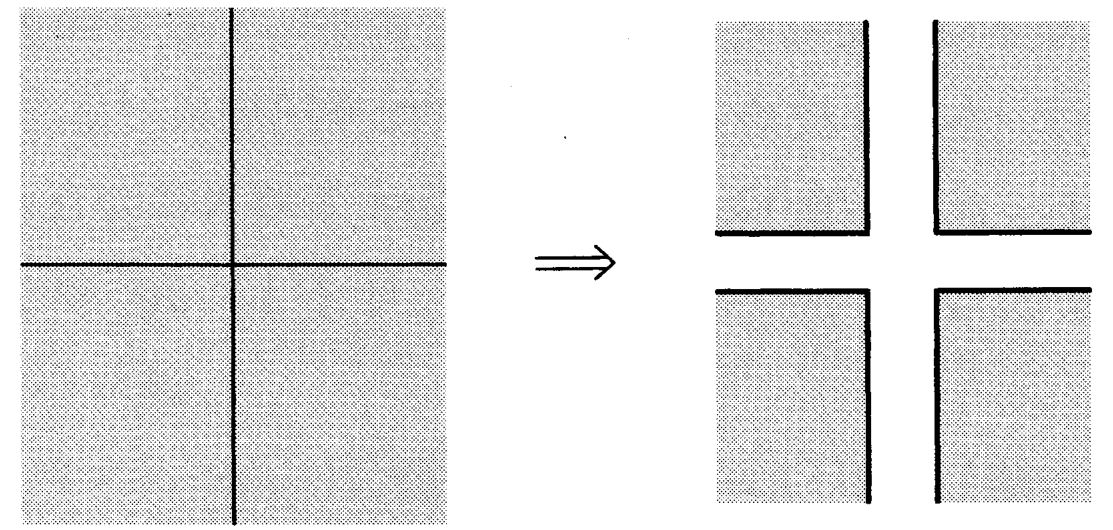
\includegraphics[width=0.55\textwidth]{figures/fig6.13.png}
    \figtitle{6.13}{化为带角流形（原书 p.325）}
  \end{figure}

% [原文 p.326]
  把这些合起来的东西记作 $\widehat{CM}_{0,k+m+1}$。存在映射 $\pi:\widehat{CM}_{0,k+m+1}\to CM_{0,k+m+1}$，使 $CM_{0,k+m+1,\ell}$ 的点关于 $\pi$ 的原像是 $(S^1)^\ell$。在 $M_{0,k+m+1}$ 上 $\pi$ 是同胚。把 $C(k,m)$ 的像在 $\widehat{CM}_{0,k+m+1}$ 中的闭包记作 $\bar C(k,m)$。

  下面确认 $\rd\psi^i_j$ 光滑延拓到 $\bar C(k,m)$。首先考虑 $k=2$、$m=2$ 的情形，即 $C(2,2)$。$C(2,2)$ 是 $[z_1,z_2,w_1,w_2]$ 的集合。可把 $z\mapsto za+b$ 的代表元取成 $w_1=0$、$w_2=1$。这样的取法唯一。因此 $C(2,2)$ 的点由 $(z_1,z_2)$ 表示。无穷远点对应 $|z_1-z_2|\to0$ 的情形，以及 $z_i\to0$、$z_i\to1$ 或 $z_i\to\infty$ 的情形。（也有其组合。）

  第 1 种情形即 $z_1=z_2$ 对应的无穷远点由 $z=z_1=z_2$ 的坐标与 $S^1$ 的元决定。这个 $S^1$ 记住 $z_1$ 从哪个方向接近 $z_2$（图 6.14(a)）。因此若 $e^1_j$ 是连接 $p_1$ 与 $p_2$ 的边，则 $\rd\psi^1_j$ 延拓到这个无穷远点。

  \begin{figure}[htbp]
    \centering
    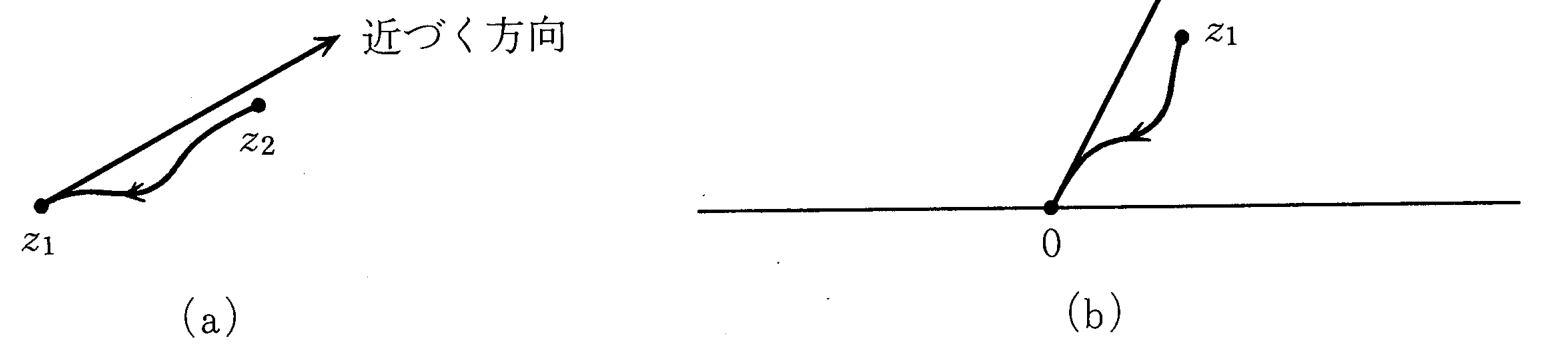
\includegraphics[width=0.78\textwidth]{figures/fig6.14.png}
    \figtitle{6.14}{$\rd\psi^i_j$ 的延拓（原书 p.326）}
  \end{figure}

  其次考虑 $z_1=w_1$ 的情形。与此对应的是决定 $z_1$ 从哪个方向接近 $w_1=0$ 的参数，对应半圆周。（这半圆周的两端连着 $z_1\in\R-\{0,1\}$ 的情形对应的边界。图 6.14(b)。）因此若 $e^1_j$ 是连接 $p_1$ 与 $q_1$ 的边，则 $\rd\psi^1_j$ 延拓到这个无穷远点。

  以上（多少作了省略）证明了 $k=2$、$m=2$ 时 $\rd\psi^i_j$ 延拓到紧化上。

  $k,m$ 一般的情形如下进行。要证 $\rd\psi^i_j$ 延拓。设 $e^i_j$ 的终

% [原文 p.327]
  点为 $p_{i'}$（$q_{i'}$ 的情形也相同）。此时由 $(z,\vec w)\mapsto(z_i,z_{i'};w_1,w_2)$ 定义 $C(k,m)\to C(2,2)$。这个映射光滑延拓到紧化上。又 $\rd\psi^i_j$ 是 $C(2,2)$ 上微分 1-形式的拉回。因此由已叙述的 $k=2$、$m=2$ 的情形可知，$\rd\psi^i_j$ 光滑延拓到紧化上。
\end{proof}

\begin{remark}{6.173}
  引理 6.172 的紧化是 Axelrod–Singer [28]、Kontsevich [217] 在 Chern–Simons 微扰理论中所用紧化的 2 维情形类似物。这个紧化是在实范畴中构成的，对复流形的类似构成见 [134]。
\end{remark}

\begin{remark}{6.174}
  紧化 $CM_{0,g}$ 与 $\mathrm{Comm}_\infty$ 结构有关。与这里所用的紧化 $\widehat{CM}_{0,g}$ 的差别，在于考虑带名点与奇点，还是考虑边界（图 6.15）。这一差别产生 $\mathrm{Comm}_\infty$ 结构与 $L_{\infty}$ 结构的差别，这一点在例如 [142] 等中也被注意到。在接触同调中，相当于边界的 $S^1$ 的参数在模空间中存活下来，因此产生 $L_{\infty}$ 结构。
\end{remark}

\begin{figure}[htbp]
  \centering
  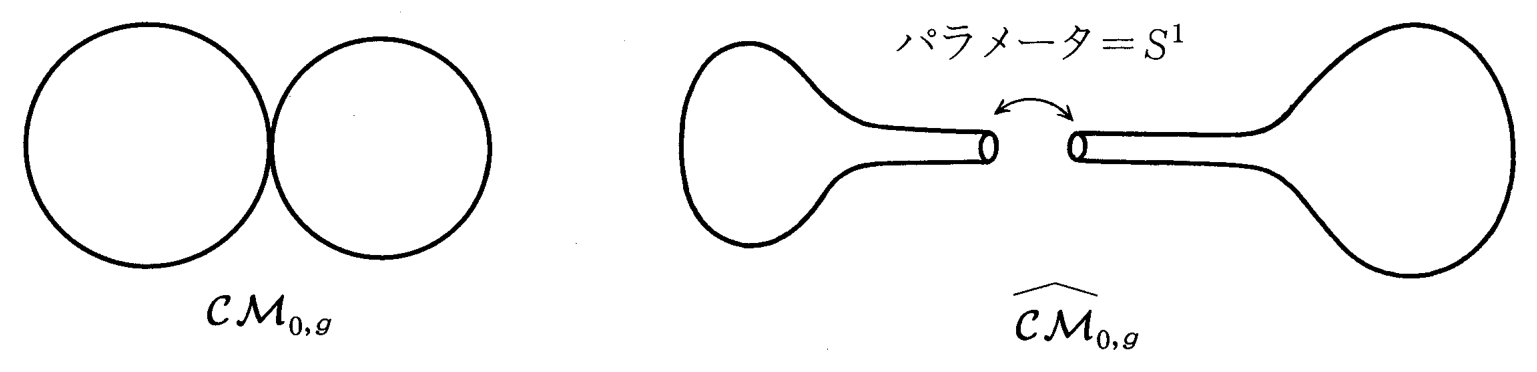
\includegraphics[width=0.78\textwidth]{figures/fig6.15.png}
  \figtitle{6.15}{$\widehat{CM}_{0,g}$（原书 p.327）}
\end{figure}

现在开始证明 $\varphi_k$ 成为 $L_{\infty}$ 写像。应证明的 $L_{\infty}$ 写像的定义式如下。
\begin{align}
  0={}&\rd\varphi_k(\alpha_1,\dots,\alpha_k) \notag\\
  &+\sum_{k_1+k_2=k}\sum_{\sigma\in\mathfrak{S}_k}\frac{\pm1}{k!}\iota_2\bigl(\varphi_{k_1}(\alpha_{\sigma(1)},\dots,\alpha_{\sigma(k_1)}),\varphi_{k_2}(\alpha_{\sigma(k_1+1)},\dots,\alpha_{\sigma(k_1+k_2)})\bigr) \notag\\
  &+\sum_{\sigma\in\mathfrak{S}_k}\frac{\pm1}{k!}\varphi_{k-1}\bigl(\iota_2(\alpha_{\sigma(1)},\alpha_{\sigma(2)}),\alpha_{\sigma(3)},\dots,\alpha_{\sigma(k)}\bigr). \tag{6.64}
\end{align}
% [Tutor Note: (6.64) 是 $L_{\infty}$ 写像的定义式：第一项是 $\varphi$ 与微分 $\rd$ 的交换子，第二项是 $\iota_2$ 与 $\varphi$ 的 Leibniz 型项，第三项是 $\varphi$ 把 $\iota_2$ 拉回。符号依赖 Koszul 约定（超对称），书中一律以 $\pm$ 略去，逐符号复现须回原论文 [221]。]
（考察 $L_{\infty}$ 代数等时，符号是与超对称性相关的本质而非

% [原文 p.328]
自明的部分，但其说明很长，故本书割爱，以 $\pm$ 等搪塞过去。）

考察在 (6.64) 的右边代入 $f_1,\dots,f_m$ 所得者。这里 $m=\sum m_i+3$，$\deg\alpha_i=m_i$。设 $\Gamma\in\mathfrak{T}(k;m_1,\dots,m_k;m)$。由 Stokes 定理，
\begin{equation}
  \int_{\partial\bar C(k,m)}\prod_{i,j}\rd\psi^i_j=0. \tag{6.65}
\end{equation}
想看由 (6.65) 导出 (6.64)。$\partial\bar C(k,m)$ 分为若干成分。它们分为图 6.16 的两种类型。即设 $(z,\vec w)\in C(k,m)$ 时，$z_i$ 中两个以上聚集到 $\HH$ 的点的情形（图 6.16 的 (A)），以及 $z_i,w_j$ 中两个以上（或一个 $z_i$）聚集到 $\R$ 的点的情形（图 6.16 的 (B)）。前者对应 (6.64) 的第 3 项，后者对应 (6.64) 的第 1 项与第 2 项。

\begin{figure}[htbp]
  \centering
  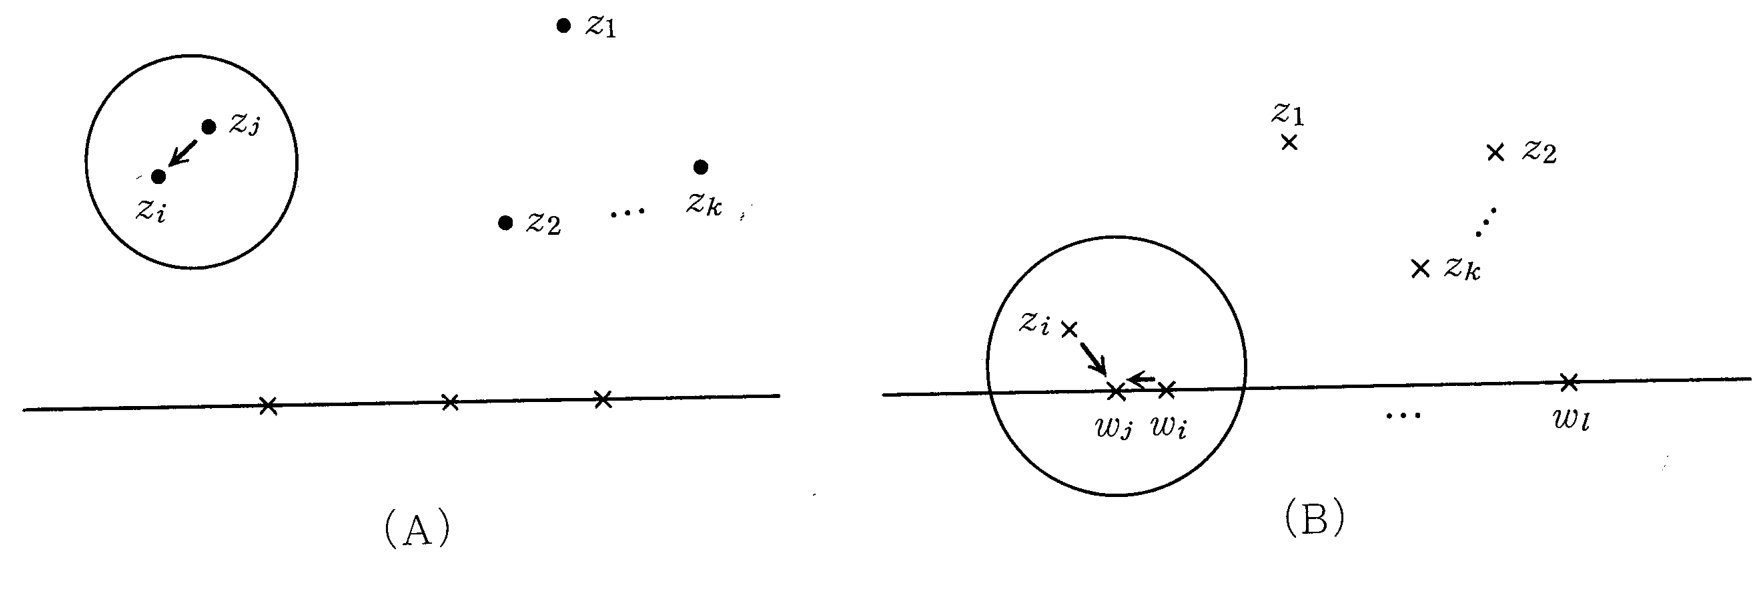
\includegraphics[width=0.90\textwidth]{figures/fig6.16.png}
  \figtitle{6.16}{$\bar C(k,m)$ 的无穷远点（原书 p.328）}
\end{figure}

在 (A) 中考虑聚集来的 $z_i$ 的个数为 2 的情形。为记号简单，设为 $z_1,z_2$。把 $\partial\bar C(k,m)$ 的相应成分记作 $\partial_{z_1=z_2}\bar C(k,m)$。若 $\Gamma$ 中连接 $p_1$ 与 $p_2$ 的边数不恰好是 1，则由维数关系，(6.65) 的对应项为 0。

设 $e^1_1$ 为以 $p_1$ 为起点、$p_2$ 为终点的边。把 $\Gamma$ 中 $e^1_1$ 缩掉、使 $p_1$ 与 $p_2$ 成为同一点所得的图记作 $\Gamma'$。考虑 (6.65) 中在 $\partial_{z_1=z_2}\bar C(k,m)$ 上积分的部分。$\partial_{z_1=z_2}\bar C(k,m)$ 是 $\bar C(k-1,m)\times S^1$，在 $S^1$ 上 $\rd\psi^1_1=\rd t$（$t\in[0,2\pi]$ 是 $S^1$ 的坐标）。因此下式 (6.66) 成立。

% [原文 p.329]
\begin{equation}
  \int_{\partial_{z_1=z_2}\bar C(k,m)}\prod_{i,j}\rd\psi^i_j
  =2\pi\int_{\bar C(k-1,m)}\prod_{(i,j)\neq(1,1)}\rd\psi^i_j. \tag{6.66}
\end{equation}
考察 $U(\Gamma')$。设 $p_1$ 与 $p_2$ 合并所得的 $\Gamma'$ 的顶点为 $p_0$。设从 $p_1$ 出发的边为 $e^1_1,\dots,e^1_{m_1}$，从 $p_2$ 出发的边为 $e^2_1,\dots,e^2_{m_2}$，则从 $p_0$ 出发的边有 $m_1+m_2-1$ 条，即 $e^2_1,\dots,e^1_{m_1},e^2_1,\dots,e^2_{m_2}$。

令
\[
  \alpha^{a(1;2),\dots,a(1;m_1),a(2;1),\dots,a(2;m_2)}_0
  =\sum_\ell\alpha^{\ell,a(1;2),\dots,a(1;m_1)}_1\partial_\ell\alpha^{a(2;1),\dots,a(2;m_2)}_2.
\]
由定义可得下述等式。
\[
  U(\Gamma')(\alpha_0,\alpha_3,\dots,\alpha_k)(f_1,\dots,f_m)=\pm U(\Gamma)(\alpha_1,\dots,\alpha_k)(f_1,\dots,f_m).
\]
把 $\alpha_0$ 与从 $p_2$ 出发的边 $e^2_1$ 的终点为 $p_1$ 的情形对应的同样项合并，就得到 Schouten 括号 $\iota_2(\alpha_1,\alpha_2)$。因此得到下述引理。

\begin{lemma}{6.175}
  \[
    \sum_\Gamma\pm\frac{(2\pi)^{-2k+m-1}}{m_1!\cdots m_k!}\int_{\partial_{z_1=z_2}\bar C(k,m)}\prod_{i,j}\rd\psi^i_j\times U(\Gamma)(\alpha_1,\dots,\alpha_k)(f_1,\dots,f_m)
  \]
  是 (6.64) 的第 3 项中 $\sigma=\mathrm{id}$ 的情形。
\end{lemma}

考虑情形 (A) 中聚集来的 $z_i$ 的个数为 3 以上的情形。把 $\partial\bar C(k,m)$ 中对应于此情形的成分记作 $\partial_{A,\ge3}\bar C(k,m)$。则下述引理成立。

\begin{lemma}{6.176}
  \[
    \int_{\partial_{A,\ge3}\bar C(k,m)}\prod_{i,j}\rd\psi^i_j=0.
  \]
\end{lemma}
% [Tutor Note: 引理 6.176 的证明是纯维数论证：$\ge3$ 个 $z_i$ 同时聚集使该边界成分的维数低于积分所需次数，故积分为零；这正是 Kontsevich 构型空间积分能只留下“二元”与“一元”贡献的原因。]

引理 6.176 的证明是定理 6.166 证明的要点之一，但省略。见 [221] §6.6。

转入情形 (B)。考虑聚集到边界上一点 $w_\infty$ 的点为 $p_1,\dots,p_{k(1)},q_1,\dots,q_{m(1)}$ 的情形。令 $k(1)+k(2)=k$，$m(1)+m(2)=m$。把 $\partial\bar C(k,m)$ 的相应部分记作 $\partial_{1,\dots,k(1);1,\dots,m(1)}\bar C(k,m)$。

$\partial_{1,\dots,k(1);1,\dots,m(1)}\bar C(k,m)$ 同型于直积 $\bar C(k(1),m(1))\times\bar C(k(2),m(2)+1)$。实际上第 2 成分由 $(z_{k(1)+1},\dots,z_k;w_\infty,w_{m(1)+1},\dots,w_m)$ 决定，第 1 成分由包含气泡部分 $(p_1,\dots,p_{k(1)},q_1,\dots,q_{m(1)})$ 的 $S^2$ 的部分、图

% [原文 p.330]
6.16(B) 中圆圈内的点 $z_*,w_*$ 们的状况决定\footnote{只要把奇点变成 $\infty$，在上半平面上作共形映射即可。}。

因此计算维数可知，除 $m_1+\dots+m_{k(1)}=2k(1)+m(1)-2$ 的情形以外，(6.65) 中在 $\partial_{1,\dots,k(1);1,\dots,m(1)}\bar C(k,m)$ 上积分的部分为 0。

进一步可知下事。

\begin{lemma*}{6.177}
  若从 $p_1,\dots,p_{k(1)}$ 中某一个出发的边，其终点是 $p_1,\dots,p_{k(1)},q_1,\dots,q_{m(1)}$ 以外的点（图 6.17），则 (6.65) 中在 $\partial_{1,\dots,k(1);1,\dots,m(1)}\bar C(k,m)$ 上积分的部分为 0。
\end{lemma*}
\begin{proof}
  设 $e^i_j$ 的起点为 $p_i$（$i\le k(1)$）、终点为 $p_{i'}$（$i'>m(1)$）。则在 $\partial_{1,\dots,k(1);1,\dots,m(1)}\bar C(k,m)$ 上，$z_i$ 是实数，且 $z_{i'}\neq z_i$，故 $\psi^i_j$ 总在 $-\pi/2$ 与 $\pi/2$ 之间（图 6.17）。特别地，$\psi^i_j$ 可取单值。因此在其中 $\rd\psi^i_j$ 是完全形式。由此得出结论。
\end{proof}

\begin{figure}[htbp]
  \centering
  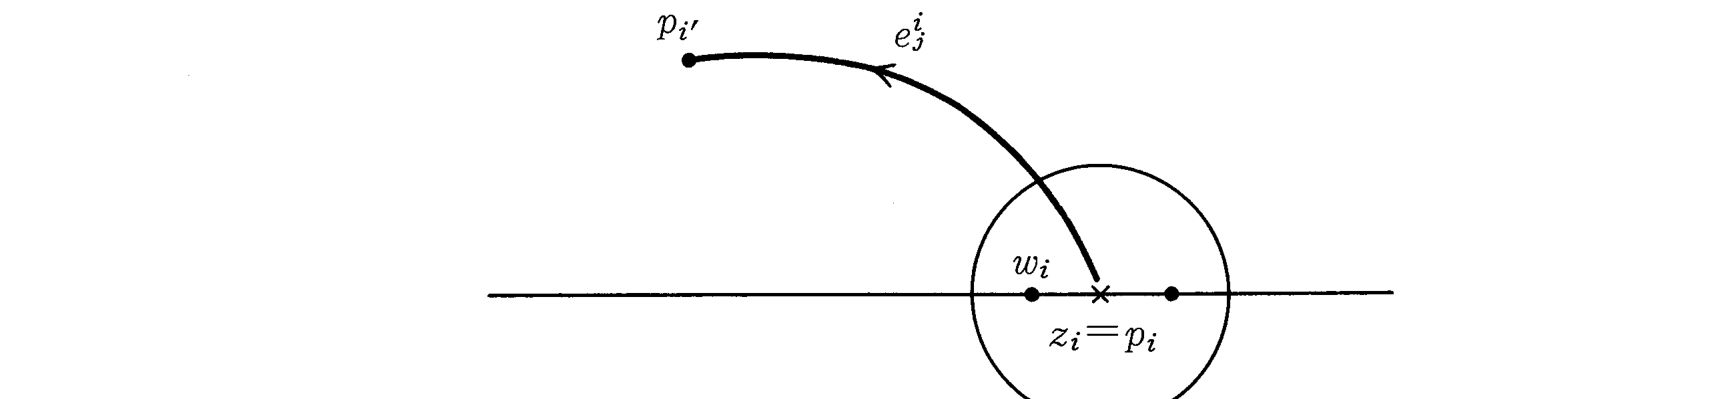
\includegraphics[width=0.80\textwidth]{figures/fig6.17.png}
  \figtitle{6.17}{$\psi^i_j$ 成为单值（原书 p.330）}
\end{figure}

现设 $m_1+\dots+m_{k(1)}=2k(1)+m(1)-2$。把 $\Gamma$ 中 $p_1,\dots,p_{k(1)},q_1,\dots,q_{m(1)}$ 以及它们之间的边全部缩成一点所得者记作 $\Gamma_2$。另一方面，以 $p_1,\dots,p_{k(1)},q_1,\dots,q_{m(1)}$ 为顶点、以连接这些顶点的 $\Gamma$ 的边为边的图记作 $\Gamma_1$。

不妨设引理 6.177 的假定不被满足。即不妨设没有以 $w_\infty$ 为起点的 $\Gamma_2$ 的边。于是 $\Gamma_2\in\mathfrak{T}(k(2),m(2)+1)$，$\Gamma_1\in\mathfrak{T}(k(1),m(1))$。下一条引理由定义立即明白。

% [原文 p.331]
\begin{lemma}{6.178}
  \[
    (2\pi)^{-(2k+m-1)}\int_{\partial_{1,\dots,k(1);1,\dots,m(1)}\bar C(k,m)}\prod_{i,j}\rd\psi^i_j=W(\Gamma_1)W(\Gamma_2).
  \]
\end{lemma}

其次考虑 $U(\Gamma)$。先考虑 $k(1)=k$、$m(1)=m-1$ 的情形（图 6.18(a)）。此时显然有
\[
  U(\Gamma)(\alpha_1,\dots,\alpha_k)(f_1,\dots,f_m)=U(\Gamma_1)(\alpha_1,\dots,\alpha_k)(f_1,\dots,f_{m-1})f_m.
\]
同样，考虑 $k(1)=0$、$m(1)=2$ 的情形（图 6.18(b)），有
\[
  U(\Gamma)(\alpha_1,\dots,\alpha_k)(f_1,\dots,f_m)=U(\Gamma_1)(\alpha_1,\dots,\alpha_k)(f_1f_2,f_3,\dots,f_m).
\]
这些正好出现在 Hochschild 上同调的边界作用素的定义中。

\begin{figure}[htbp]
  \centering
  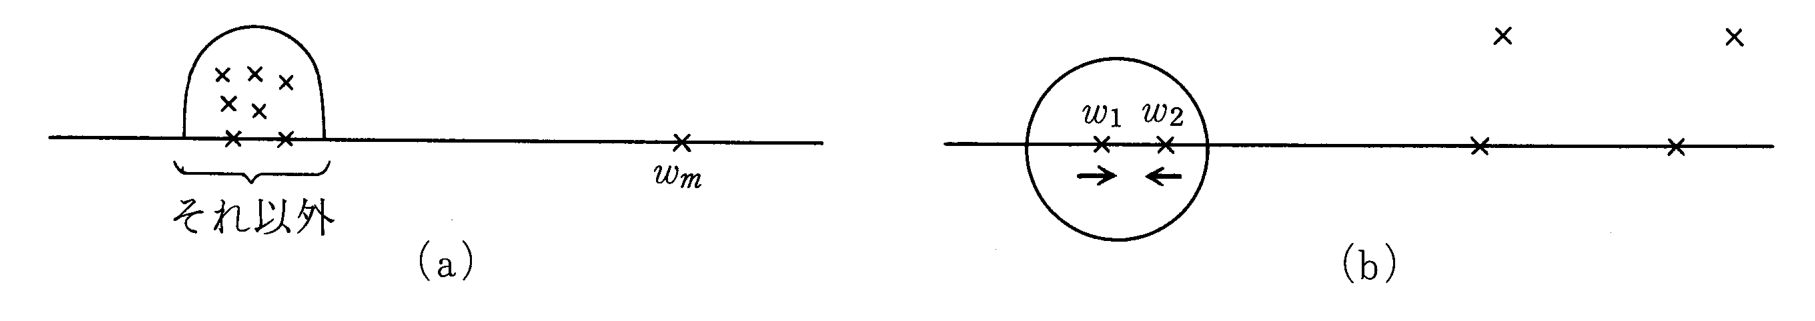
\includegraphics[width=0.82\textwidth]{figures/fig6.18.png}
  \figtitle{6.18}{Hochschild 上同调的边界作用素（原书 p.331）}
\end{figure}

因此得到下述引理 6.179。

\begin{lemma}{6.179}
  满足 $k(1)=0,m(1)=2$ 或 $k(2)=0,m(2)=1$ 的、(6.65) 的 (B) 型边界成分对应的项之和，与 $U(\Gamma)(\alpha_1,\dots,\alpha_k)(f_1,\dots,f_m)$ 之积，给出 (6.64) 的第 1 项。
\end{lemma}

考虑引理 6.179 中出现的情形以外的 $\Gamma_1,\Gamma_2$。此时令
\[
  g=U(\Gamma_1)(\alpha_1,\dots,\alpha_{k(1)})(f_1,\dots,f_{m(1)}),
\]
则
\[
  U(\Gamma)(\alpha_1,\dots,\alpha_k)(f_1,\dots,f_m)=U(\Gamma_2)(\alpha_{k(1)+1},\dots,\alpha_k)(g,f_{m(1)+1},\dots,f_m).
\]
因此，用 $W(\Gamma_1)W(\Gamma_2)$ 乘它所得者，给出合成
\[
  U(\Gamma_2)(\alpha_{k(1)+1},\dots,\alpha_k)\circ U(\Gamma_1)(\alpha_1,\dots,\alpha_{k(1)})(f_1,\dots,f_m)
\]
的一个项。于是由引理 6.178 与 Gerstenhaber 括号的定义，得到下述引理 6.180。

% [原文 p.332]
\begin{lemma}{6.180}
  (6.65) 的 (B) 型边界成分对应的项中，不满足引理 6.177 的假定者之和，与 $U(\Gamma)(\alpha_1,\dots,\alpha_k)(f_1,\dots,f_m)$ 之积，给出 (6.64) 的第 2 项。
\end{lemma}

由引理 6.175、6.176、6.177、6.179、6.180 与式 (6.65)，(6.64) 成立。即 $\varphi_k$ 确定 $L_{\infty}$ 写像。虽然省略了符号等若干部分，以上是定理 6.166（$\R^n$ 情形）证明的概要。

定理 6.166 与定理 6.157 组合，被预告可应用于镜像对称（[221]），但除 [32] 中数行的记述以外似乎尚未发表。读 [216] 的话，这两个定理的关系多少能看出来。

定义 6.171 的用费曼路径积分的表示由 [58] 给出。变形量子化的具体表示被详细考察过的例子并不多。$\C^n$ 上辛结构由常系数微分 2-形式给出的情形，有称为 Moyal 积（Moyal product）的具体表示。即令
\[
  \{f,g\}=\sum_{i,j}\omega^{ij}\partial_{x_i}f\partial_{x_j}f,
\]
则得到下式 (6.67)。
\begin{equation}
  f\star_Tg=\sum_k\frac{T^k}{k!}(\omega^{ij}\partial_{x_i}\partial_{y_j})^kf(x)g(y)\Big|_{x=y}. \tag{6.67}
\end{equation}
% [Tutor Note: (6.67) 是 Moyal 积（Weyl 量子化）；其与 (1.8) 的差别只是 $\sqrt{-1}$ 与 $\hbar$ 的约定。书中把 $T$ 当形式不定元、把 $\hbar$ 也暂当不定元看待，故形式幂级数范围内两种写法等价；若讨论收敛性则不等价。]

把形变量子化不作为 $T$ 的形式幂级数、而作为代入 $T$ 的值的收敛幂级数来讨论，仍在研究途中\footnote{一个问题是：代入 $T$ 的值后 $f\star g$ 成为关于 $f,g$ 的无限阶微分作用素，与有限阶微分作用素不同，不再具有局部性。（局部性是指 $f\star g$ 在 $p$ 处的值只由 $f,g$ 及其微分在 $p$ 处的值决定。）}。(6.67) 与例如 [34] 等的写法之间有 $2\sqrt{-1}T=\hbar$ 的关系。（$\hbar$ 是 Planck 常数，但暂且看作不定元。）只要在形式幂级数的范围内考虑，有没有 $\sqrt{-1}$ 都不大有差别，但用收敛幂级数考虑时会产生大的差别。看 (1.8) 的话，有 $\sqrt{-1}$ 大概更自然。令 $\Omega(u,v)=\sum\omega^{ij}u_iv_j$，则 (6.67) 成为

% [原文 p.333]
\begin{equation}
  f\star_\hbar g(z)=\int\exp\bigl(\sqrt{-1}\,\hbar\,\Omega(z-x,z-y)\bigr)f(x)g(y)\,\rd x\rd y \tag{6.68}
\end{equation}
（见 [34]）。

% CHUNK ch06c2 DONE
